\documentclass[a3paper, 16pt]{article}
\usepackage[inkscapepath=../barcodes_out/dummy/pdf/inkscape_out/]{svg}
\usepackage{tikz}
\usetikzlibrary{fadings}
\usepackage{float}
\usepackage{graphicx}
\usepackage{pdflscape}
\usepackage[a3paper, left=0.5cm, right=0.5cm, top=0.5cm, bottom=0.5cm]{geometry}
\usepackage{background}
\usepackage[T1]{fontenc}
\usepackage{txfonts}

\svgpath{{../barcodes_out/dummy/svg/}}

\tikzfading[name=custom fade,
    inner color=transparent!0,
    outer color=transparent!50]

% Define the background image
\backgroundsetup{
    scale=1,
    color=black,
    opacity=0.4,
    angle=90,
    position=current page.center,
    vshift=0cm,
    contents={%
    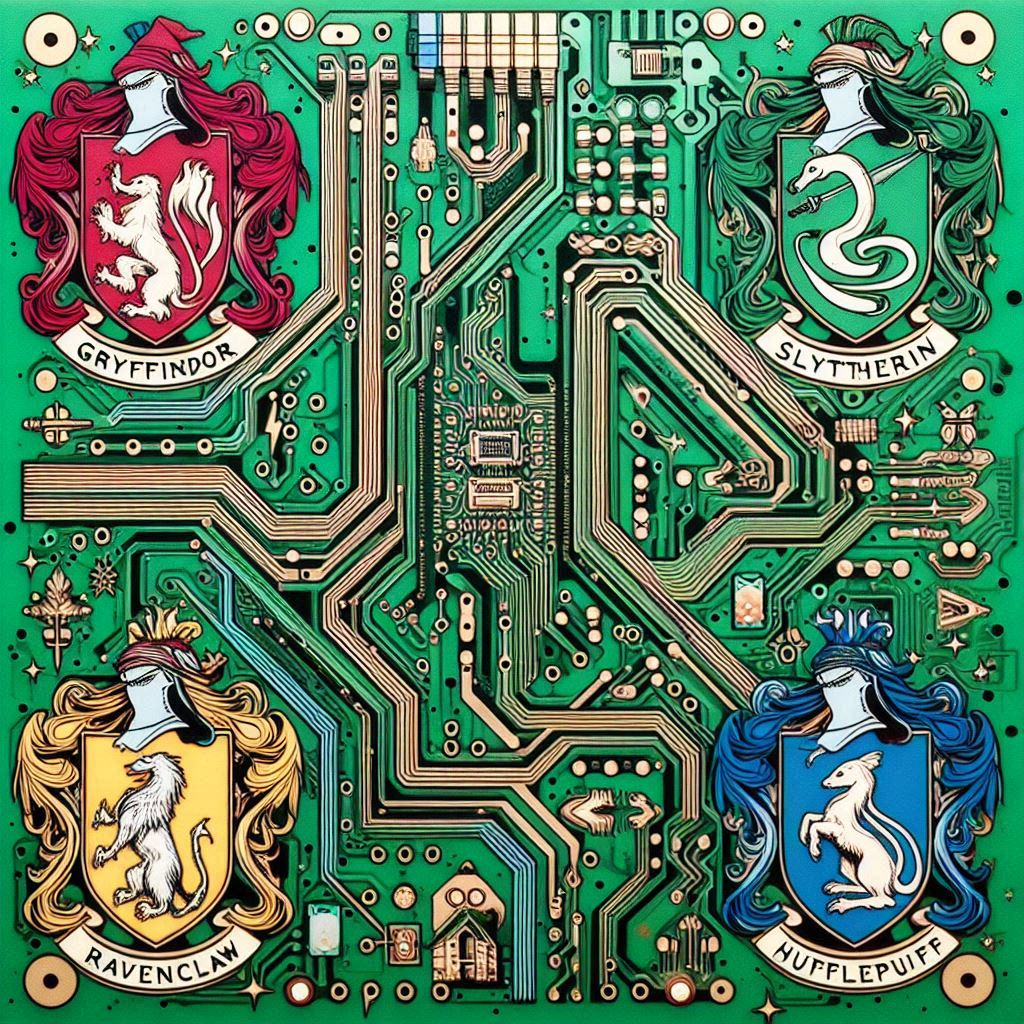
\includegraphics[width=0.99\paperheight,height=0.7\paperheight]{../assets/dummy_background}%
    }
}

\begin{document}
    \begin{landscape}

        
\begin{tikzpicture}[remember picture, overlay]
            %\fill [white,path fading=custom fade] (20,-14.5) ellipse (20cm and 7cm);
            \fill [white,path fading=circle with fuzzy edge 10 percent] (20,-14.5) ellipse (20cm and 7cm);
        \end{tikzpicture}

        \vspace*{\fill}
        \thispagestyle{empty}
        \begin{center}
            \textbf{\Huge \textbf{AUFBAU EINES BARCODES}}
        \end{center}

        \begin{figure}[!h]
            \centering
            \begin{tikzpicture}
                \node[anchor=south west, inner sep=0] (barcode) at (0,0) {\includesvg[scale=0.38]{\VAR{ file }}};
                \begin{scope}
                    [x={(barcode.north west)}, y={(barcode.south east)}]
                    \BLOCK{ for numeral in dummy }
                    \BLOCK{ set word = dimensions[loop.index0] }
                    \BLOCK{ set position = 0.005 + (0.01 * loop.index0) }
                    \BLOCK{ set position = position|round(3) }
                    # if numeral == 0
                    \node[anchor=west, text=white, rotate=90] at (-0.007, \VAR{ position }) {\textbf{\VAR{ word }}};
                    # elif numeral == 1
                    \node[anchor=west, rotate=90] at (-0.007, \VAR{ position }) {\textbf{\VAR{ word }}};
                    # endif
                    \BLOCK{ endfor }
                \end{scope}
            \end{tikzpicture}
        \end{figure}

% Legend
        \begin{tikzpicture}[overlay]
            \node[anchor=south west] at ([xshift=10cm, yshift=-7cm]barcode.north west) {
                \begin{minipage}{\textwidth}
                    \begin{tikzpicture}
                        \draw[fill=yellow, draw=black] (0,0) rectangle (1,0.5);
                        \node[right] at (1.2,0.25) {\huge Wort in Absatz enthalten};
                        \draw[fill=black, draw=black] (9.5,0) rectangle (10.5,0.5);
                        \node[right] at (10.7,0.25) {\huge \color{black} Wort nicht in Absatz enthalten};
                    \end{tikzpicture}
                \end{minipage}
            };
        \end{tikzpicture}
        \vspace*{\fill}

    \end{landscape}
\end{document}
